\chapter{Evaluation}\label{chap:evaluation}

The goal of (dynamic) texture synthesis is to generate 
samples that are indistinguishable from the real input target
texture by a human observer.
In this chapter, a variety of synthesis results are presented,
including qualitative comparisons with extant methods and a user study to quantitatively evaluate the realism
of the synthesized results.
Given their temporal nature, the results are best viewed as 
videos, which are available on the project page: \url{ryersonvisionlab.github.io/two-stream-projpage}.
The two-stream architecture was implemented using TensorFlow
\cite{tabadi2015tensorflow}, an open source machine learning framework.
Results were generated using an NVIDIA Titan X (Pascal) GPU
and synthesis times ranged between one to three hours (corresponding to $6,000$ optimization iterations)
to generate $12$ frames with an image resolution of 
$256 \times 256$.
For the full synthesis results and source code, please refer to the
supplemental material available on the project page.

\section{Qualitative results}\label{sec:qualitative_results}

In this section, a qualitative analysis is performed on the tasks of dynamic texture synthesis, incremental texture synthesis,
temporally-endless texture synthesis, and dynamics style transfer.

\subsection{Dynamic texture synthesis}

The dynamic texture synthesis process was applied 
to a wide range of textures selected from the 
DynTex \cite{peteri2010} database and others that were collected in-the-wild.
The collected textures include ones that adhere to the texture assumptions of this thesis (\ie, spatiotemporal homogeneity) and ones that do not.
Included in the supplemental material are synthesized results
of nearly 60 different textures that encapsulate a range of
phenomena, such as flowing water, waves, clouds, fire, rippling
flags, waving plants, and schools of fish.
Some sample frames are shown in Fig.\ \ref{fig:successes_1} and Fig.\ \ref{fig:successes_2}
but readers are encouraged to view the videos to fully appreciate
the results.

Fig.\ \ref{fig:successes_1} and Fig.\ \ref{fig:successes_2} show some example success cases with the
two-stream method where appearance and dynamics characteristics from the
target are reliably preserved in the synthesized result. The
upward fiery dynamics and flickering appearance of \path{fireplace_1}, the outward dynamics of the explosive splash of \path{lava},
the wispy fluid dynamics of \path{smoke_1}, the
flowing vegetation in \path{underwater_vegetation_1}, and the downward 
rippling flow of \path{water_3}.

\clearpage
\begin{figure*}[t!]
\begin{center}
\begin{tabular}{ >{\centering\arraybackslash} m{0.16\textwidth} || >{\centering\arraybackslash} m{0.80\textwidth} }

{\footnotesize \path{fireplace_1}\break(original)} &
\showtexture{fireplace_1/frame_} \\
\hline
{\footnotesize \path{fireplace_1}\break(synthesized)} &
\showtexture{fireplace_1_output/frame_} \\

\hline \hline
{\footnotesize \path{lava}\break(original)} &
\showtexture{lava/frame_} \\
\hline
{\footnotesize \path{lava}\break(synthesized)} &
\showtexture{lava_output/frame_} \\

\hline \hline
{\footnotesize \path{smoke_1}\break(original)} &
\showtexture{smoke_1/frame_} \\
\hline
{\footnotesize \path{smoke_1}\break(synthesized)} &
\showtexture{smoke_1_output/frame_} \\

%\hline \hline
%{\footnotesize \path{underwater_vegetation_1}\break(original)} &
%\showtexture{underwater_vegetation/frame_} \\
%\hline
%{\footnotesize \path{underwater_vegetation_1}\break (synthesized)} &
%\showtexture{underwater_vegetation_output/frame_} \\
%
%\hline \hline
%{\footnotesize \path{water_3}\break(original)} & 
%\showtexture{water_3/frame_} \\
%\hline
%{\footnotesize \path{water_3}\break(synthesized)} & 
%\showtexture{water_3_output/frame_} \\
\end{tabular}
\end{center}
\vspace{-0.45cm}
\caption[Dynamic texture synthesis success examples]{Dynamic texture synthesis success examples. Names correspond to files in the supplemental material.}
 \label{fig:successes_1}
\end{figure*}

\begin{figure*}[t!]
\begin{center}
\begin{tabular}{ >{\centering\arraybackslash} m{0.16\textwidth} || >{\centering\arraybackslash} m{0.80\textwidth} }
{\footnotesize \path{underwater_vegetation_1}\break(original)} &
\showtexture{underwater_vegetation/frame_} \\
\hline
{\footnotesize \path{underwater_vegetation_1}\break (synthesized)} &
\showtexture{underwater_vegetation_output/frame_} \\

\hline \hline
{\footnotesize \path{water_3}\break(original)} & 
\showtexture{water_3/frame_} \\
\hline
{\footnotesize \path{water_3}\break(synthesized)} & 
\showtexture{water_3_output/frame_} \\
\end{tabular}
\end{center}
\vspace{-0.45cm}
\caption[Dynamic texture synthesis success examples]{Dynamic texture synthesis success examples. Names correspond to files in the supplemental material.}
 \label{fig:successes_2}
\end{figure*}

\clearpage

\subsubsection{Failure modes}

Example failure modes of the two-stream method are presented in Fig.\ 
\ref{fig:failures}.
In general, most failures result from inputs that
violate the underlying assumption of a dynamic texture, \ie, 
the appearance and/or dynamics are not spatiotemporally homogeneous.
In the case of the \path{escalator} example, the long edge 
structures in the appearance are not spatially homogeneous, 
and the dynamics vary due to perspective effects that
change the motion from purely downward to downward and outward.
The resulting synthesized texture captures an overall downward 
motion but lacks the perspective effects and is unable to 
consistently reproduce the long edge structures.
This is consistent with previous observations
on static texture synthesis \cite{gatys2015} and suggests it is a 
limitation of the Gram matrix representation used
in the appearance stream.

Another example is the \path{flag} sequence where the rippling 
dynamics are relatively homogeneous across the pattern but the 
appearance varies spatially.
As expected, the generated texture does not faithfully
reproduce the appearance; however, it does exhibit plausible 
rippling dynamics.

Also shown in Fig.\ \ref{fig:failures} is the \path{cranberries} sequence, which consists of a combination of swirling and wave dynamics.
The model faithfully reproduces the appearance
but is unable to capture the spatially varying dynamics.
Interestingly, it still produces a result
which is statistically indistinguishable from real in the user 
study discussed in Sec.\ \ref{sec:user_study}.

\clearpage
\begin{figure}[t]
\begin{center}
\begin{tabular}{ >{\centering\arraybackslash} m{0.16\textwidth} || >{\centering\arraybackslash} m{0.80\textwidth} }
{\footnotesize \path{escalator}\break(original)} & 
\showtexture{escalator/frame_} \\
\hline
{\footnotesize \path{escalator}\break(synthesized)} & 
\showtexture{escalator_output/frame_} \\
\hline \hline
{\footnotesize \path{flag}\break(original)} &
\showtexture{flag/frame_} \\
\hline
{\footnotesize \path{flag}\break(synthesized)} &
\showtexture{flag_output/frame_} \\
\hline \hline
{\footnotesize \path{cranberries}\break(original)} &
\showtexture{cranberries/frame_} \\
\hline
{\footnotesize \path{cranberries}\break(synthesized)} &
\showtexture{cranberries_output/frame_} \\
\end{tabular}
\end{center}
\vspace{-0.45cm}
\caption[Dynamic texture synthesis failure examples.]{Dynamic texture synthesis failure examples. In
these cases, the failures are attributed to either the
appearance or the dynamics not being homogeneous.}
\label{fig:failures}
\end{figure}
\clearpage

\subsubsection{Appearance vs.\ dynamics streams}

Two experiments were conducted to verify that the appearance and dynamics
streams were capturing complementary information.
To validate that the texture generation of multiple frames
would not induce dynamics consistent with the input, frames were generated
starting from randomly generated noise but only using the
appearance statistics and corresponding loss, \ie,
Eq.\ \ref{eq:apploss}.
As expected, this produced frames that were valid textures but
with no coherent dynamics present.
To examine the dynamics, see 
\path{fish} in the supplemental material.

Similarly, to validate that the dynamics stream did not 
inadvertently include appearance information, dynamic textures were synthesized
using the dynamics loss only, \ie, Eq.\ \ref{eq:dynloss}.
The resulting frames had no visible appearance and had
an extremely low dynamic range, \ie, the standard
deviation of pixel intensities was 10 for values in $[0,255]$.
This indicates a general invariance to appearance and 
suggests that the two-stream dynamic texture representation
has factored appearance and dynamics, as desired.
Results for a sequence containing a school of fish are shown in
Fig.\ \ref{fig:appearance_only_vs_dynamics_only} with enhanced contrast.

\begin{figure}[t]
\begin{center}
\begin{tabular}{ >{\centering\arraybackslash} m{0.16\textwidth} || >{\centering\arraybackslash} m{0.80\textwidth} }
{target (\path{fish})} & 
\showtexture{fish/frame_} \\
\hline \hline
{appearance only} &
\showtexture{fish_spatialonly/frame_} \\
\hline
{dynamics only} &
\showtexture{fish_dynamicsonly/frame_} \\
\hline
{both streams} & 
\showtexture{fish_output/frame_} \\
\end{tabular}
\end{center}
\vspace{-0.45cm}
\caption[Two-stream dynamic texture synthesis versus dynamics-only and appearance-only texture synthesis]{Two-stream dynamic texture synthesis versus dynamics-only and appearance-only texture synthesis.
(top row) Target dynamic texture.
(second row)
Texture synthesis without dynamics constraints shows
consistent per-frame appearance but no temporal coherence.
(third row)
Texture synthesis without appearance constraints shows
limited per-frame appearance with pixel intensities having a standard deviation of 10.
(bottom row)
Including both streams induces consistent appearance and dynamics.
}
\label{fig:appearance_only_vs_dynamics_only}
\end{figure}



\subsection{Incremental texture synthesis}

Dynamic textures synthesized incrementally, as described in Sec.\
\ref{sec:incremental_synthesis}, are included in the supplemental.
Sequences as long as 122 frames (using 11 frame subsequences) were synthesized
with no observed divergence or degradation. The resulting textures were 
perceptually indistinguishable from those synthesized with the typical batch process.

\subsection{Temporally-endless texture synthesis}

An example of a synthesized temporally-endless dynamic texture is shown in
Fig.\ \ref{fig:temporally_endless_synthesis}. As described in Sec.\ 
\ref{sec:temporally_endless_synthesis}, the dynamic texture appears
temporally endless, \ie, there is no apparent temporal discontinuity between the last and first frames.

\begin{figure}[t]
	\centering
    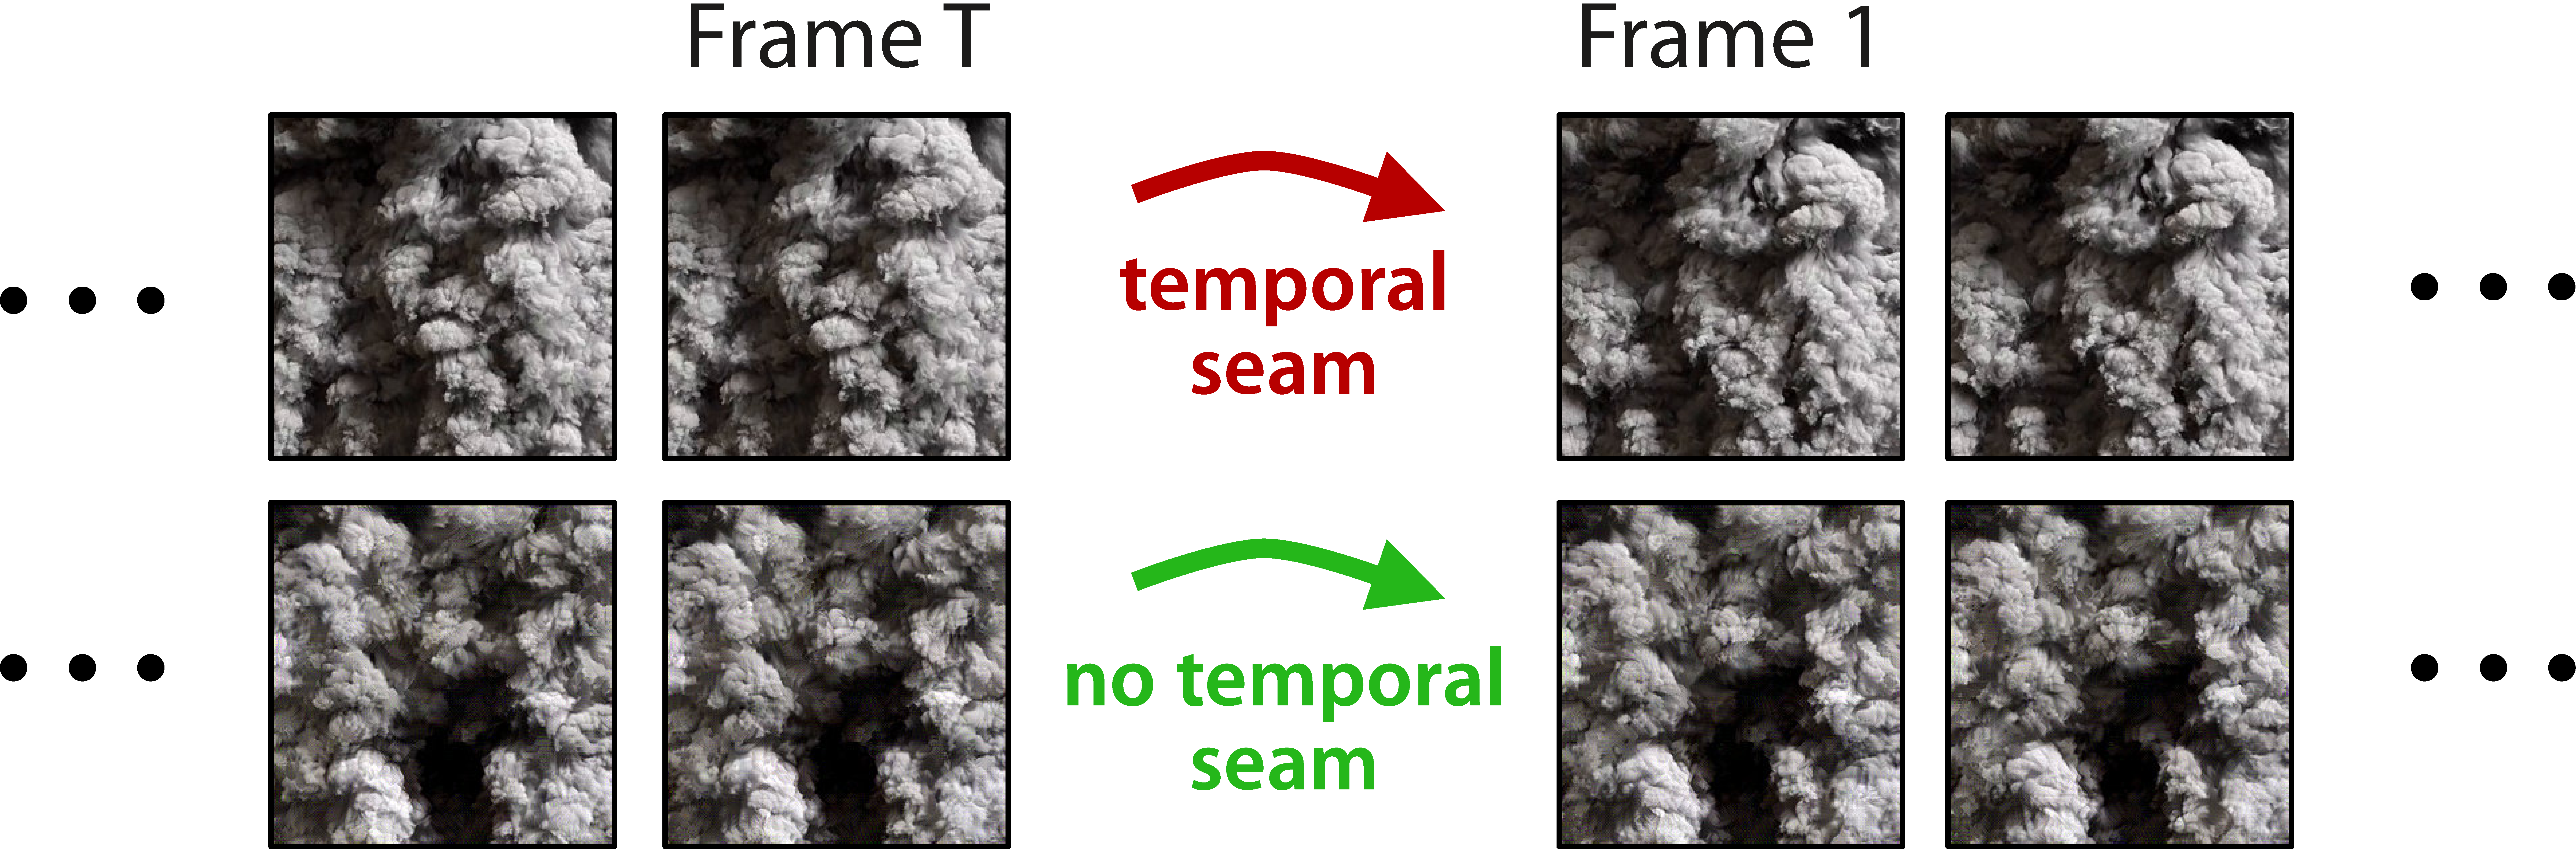
\epsfig{file=temporally_endless_synthesis.pdf, width = 0.9\textwidth}
	\caption[Temporally-endless texture synthesis.]{Temporally-endless texture synthesis. (top row) Target texture. (bottom row) Synthesized texture.
	 By adding an additional loss to the dynamics stream that ties the last frame to the first, the synthesized dynamic texture appears to be temporally endless. Note the lack of an abrupt appearance change (\ie, temporal seam) between the last frame and the first frame of the synthesized dynamic texture.}
	\label{fig:temporally_endless_synthesis}
\end{figure}



\subsection{Dynamics style transfer}

A dynamics style transfer results is shown in Fig.\ 
\ref{fig:motiontransfer} (top row), using two real videos as the appearance and dynamics target, respectively.
Additional examples are available in the supplemental material.
When performing dynamics style transfer it is important
that the appearance structure of both targets to be similar in scale and semantics,
otherwise, the generated dynamic textures will look unnatural.
For instance, transferring the dynamics of a flame onto a water 
scene will generally produce implausible results (Fig.\ \ref{fig:bad_motiontransfer}).

\begin{figure}[t]
\begin{center}
\begin{tabular}{>{\centering\arraybackslash} m{0.16\textwidth} || >{\centering\arraybackslash} m{0.80\textwidth} }
appearance target &
synthesized output \\
\hline \hline
\vspace{0.1cm}\showtexframe{water_paint.jpeg} &
\showtexture{fireplace_1_to_water_paint_output/frame_} \\
\end{tabular}
\end{center}
\vspace{-0.45cm}
\caption[Dynamics style transfer with incompatible appearance and dynamics targets]{Dynamics style transfer with incompatible appearance and dynamics targets. The dynamics from \path{fireplace_1} are unsuccessfully transferred to a painting of ocean water.}
\label{fig:bad_motiontransfer}
\end{figure}



The dynamics of a texture can also be applied to a static input image,
as the target Gram matrices for the appearance loss can be computed
on just a single frame.
This allows us to effectively animate regions of a static image.
The result of this process can be striking and is visualized in
Fig.\ \ref{fig:motiontransfer} (second, third, and bottom rows), where the appearance is 
taken from a painting and the dynamics from a real world video.

\clearpage
\begin{figure}[t]
\begin{center}
\begin{tabular}{ >{\centering\arraybackslash} m{0.16\textwidth} || >{\centering\arraybackslash} m{0.80\textwidth} }
appearance target &
synthesized output \\
\hline \hline
\vspace{0.1cm}\showtexframe{water_img.jpeg} &
\showtexture{water_4_to_water_img_output/frame_} \\
\hline
\vspace{0.1cm}\showtexframe{fire_paint.jpeg} &
\showtexture{fireplace_1_to_fire_paint_output/frame_} \\
\end{tabular}
\end{center}
\vspace{-0.45cm}
\caption[Dynamics style transfer.]{Dynamics style transfer.
(top row) 
Appearance of still water was
used with the dynamics of a different water dynamic texture
(\path{water_4}).
(bottom row) 
The appearance of a painting of fire was used
with the dynamics of a real fire (\path{fireplace_1}).
Animated results and additional examples are available in
the supplemental material.} 
\label{fig:motiontransfer}
\end{figure}
\clearpage

\section{User study}\label{sec:user_study}

Quantitative evaluation for (dynamic) texture synthesis is a particularly
challenging task as there is no single correct output when 
synthesizing new samples of a texture.
Like in other image generation tasks (\eg, rendering), 
human perception is ultimately the most important measure.
Thus, a user study was performed to evaluate the perceived 
realism of the synthesized dynamic textures.

Similar to previous image synthesis work (\eg, \cite{chen2017}), 
a perceptual experiment was conducted with human observers to 
quantitatively evaluate the synthesis results.
A two-way alternative forced-choice (2AFC) evaluation was employed on Amazon Mechanical
Turk (AMT) with 200 different users. Each user performed 59
pairwise comparisons between a synthesized dynamic texture and 
its target.
Users were asked to choose which dynamic texture appeared more realistic
after viewing the textures independently (with a brief delay between viewing each texture) for an exposure time sampled
randomly from discrete intervals between 0.3 and 4.8 seconds.
Measures were taken to control the experimental conditions and
minimize the possibility of low quality data.
Appendix \ref{sec:experimental_procedure} provides further experimental
details of the user study.

For comparison, a baseline was constructed by using the 
flow decode layer in the dynamics loss of Eq.\ \ref{eq:dynloss}.
This corresponds with attempting to mimic the optical flow 
statistics of the texture directly.
Textures were synthesized with this model and the user study
was repeated with an additional 200 users.
To differentiate between the models, ``Flow decode layer'' 
and ``Concat layer'' are labelled in the figures to describe the
baseline and final model, respectively. An example comparing a dynamic texture synthesized on the baseline and final model is shown in Fig.\ \ref{fig:baseline_comparison}.

\begin{figure}[t]
\begin{center}
\begin{tabular}{ >{\centering\arraybackslash} m{0.16\textwidth} || >{\centering\arraybackslash} m{0.80\textwidth} }
{target (\path{waterfall})} & 
\showtexture{waterfall/frame_} \\
\hline \hline
{flow decode layer (baseline)} &
\showtexture{waterfall_flowdecode/frame_} \\
\hline
{concatenation layer (final)} & 
\showtexture{waterfall_concat/frame_} \\
\end{tabular}
\end{center}
\vspace{-0.45cm}
\caption[Comparison with a dynamic texture synthesized using optical-flow directly]{Comparison with a dynamic texture synthesized using optical-flow directly.
(top row) Target dynamic texture.
(middle row)
Dynamic texture synthesis when using the ``Flow decode layer'' on the dynamics stream. This is the baseline model and corresponds to attempting to mimic the optical flow statistics of the texture directly. The dynamics of the waterfall are poorly captured, lacking the downward motion exhibited by the target.
(bottom row)
Dynamic texture synthesis when using the ``Concat layer'' on the dynamics stream. This is the final model. The downward motion and overall dynamics of the target are reliably captured.
}
\label{fig:baseline_comparison}
\end{figure}



The results of this study are summarized in
Fig.\ \ref{fig:pairwise_alltextures} which shows user accuracy in
differentiating real versus generated textures as a function of
time for both methods. Accuracies are reported with a $95\%$ confidence level, \ie, a margin of error that is between $\pm 1.96$ standard deviations from the mean ($p$-value of $0.05$).
Overall, users are able to correctly identify the real texture
$66.1\% \pm 2.5\%$ of the time for brief 
exposures of 0.3 seconds.
This rises to $79.6\% \pm 1.1\%$ with exposures of 1.2 seconds 
and higher.
Note that ``perfect'' synthesis results would have an accuracy
of $50\%$, indicating that users were unable to differentiate 
between the real and generated textures and higher accuracy 
indicating less convincing textures.

\begin{figure}[t]
	\centering
    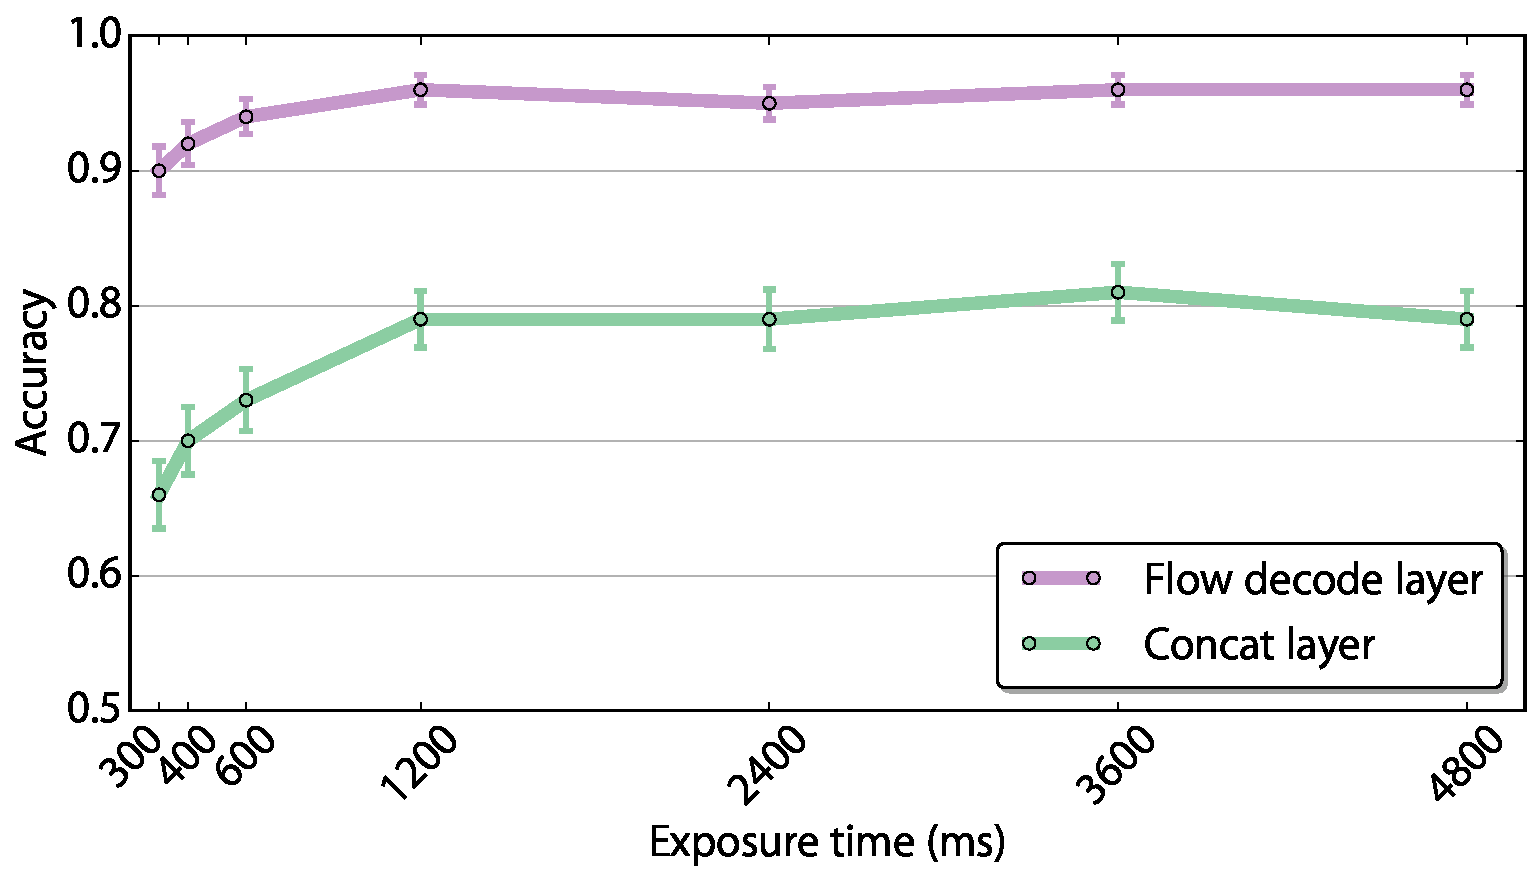
\epsfig{file=alltextures_approvedworkers.pdf, width = 0.9\textwidth}
	\caption[Time-limited pairwise comparisons across all textures]{Time-limited pairwise comparisons across all textures with $95\%$ statistical confidence intervals.}
	\label{fig:pairwise_alltextures}
\end{figure}



The results clearly show that the use of the concatenation 
layer's activations is far more effective than the flow decode 
layer.
This is not surprising as optical flow alone is known to be 
unreliable on many textures, particularly those with
translucent and/or chaotic dynamics (\eg, water, smoke, flames, etc.). Specifically, its assumptions of a single coherent movement for each pixel and brightness constancy are violated.
Also evident in these results is the time-dependant nature of 
perception for textures from both models.
Users' ability to identify the generated texture improved as 
exposure times increased to 1.2 seconds and remained relatively 
flat for longer exposures.

To better understand the performance of the proposed approach,
the results were grouped and analyzed in terms of
appearance and dynamics characteristics.
For appearance, the taxonomy
presented in \cite{lin2006quantitative} was used to group textures as
either regular/near-regular (\eg, periodic tiling and brick wall), 
irregular (\eg, a field of flowers), or
stochastic/near-stochastic (\eg, tv static or water).
For dynamics, the textures were grouped as either 
spatially-consistent (\eg, closeup of rippling sea water) or 
spatially-inconsistent (\eg, rippling sea water juxtaposed 
with translating clouds in the sky).
Results based on these groupings can be seen in
Fig.\ \ref{fig:pairwise_grouped}.

\begin{figure}[t]
	\centering
	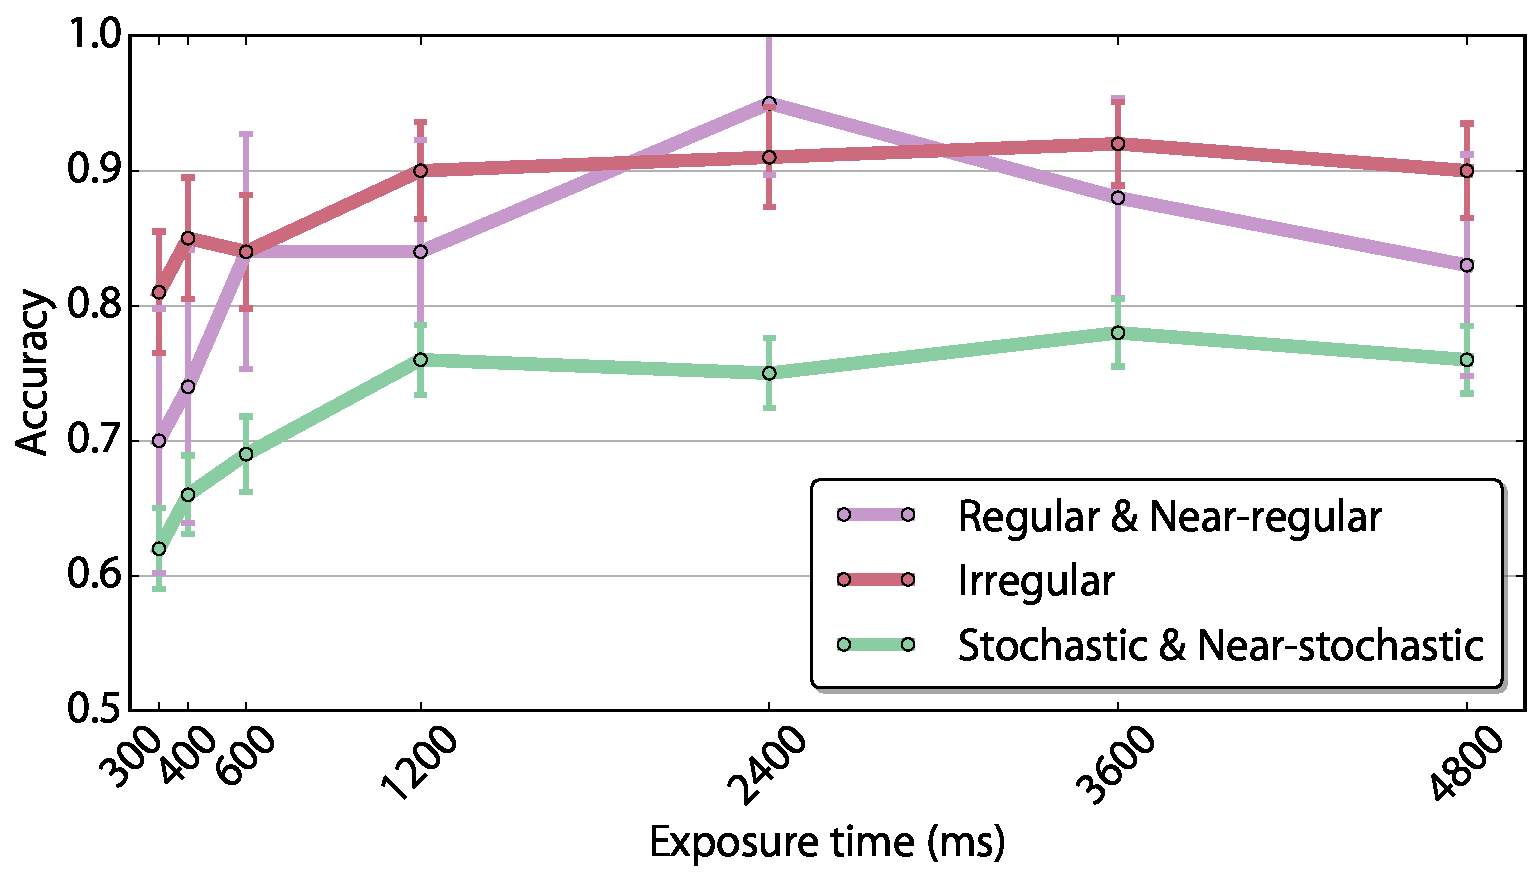
\epsfig{file=concat_appearance.pdf, width = 0.9\textwidth}\\
    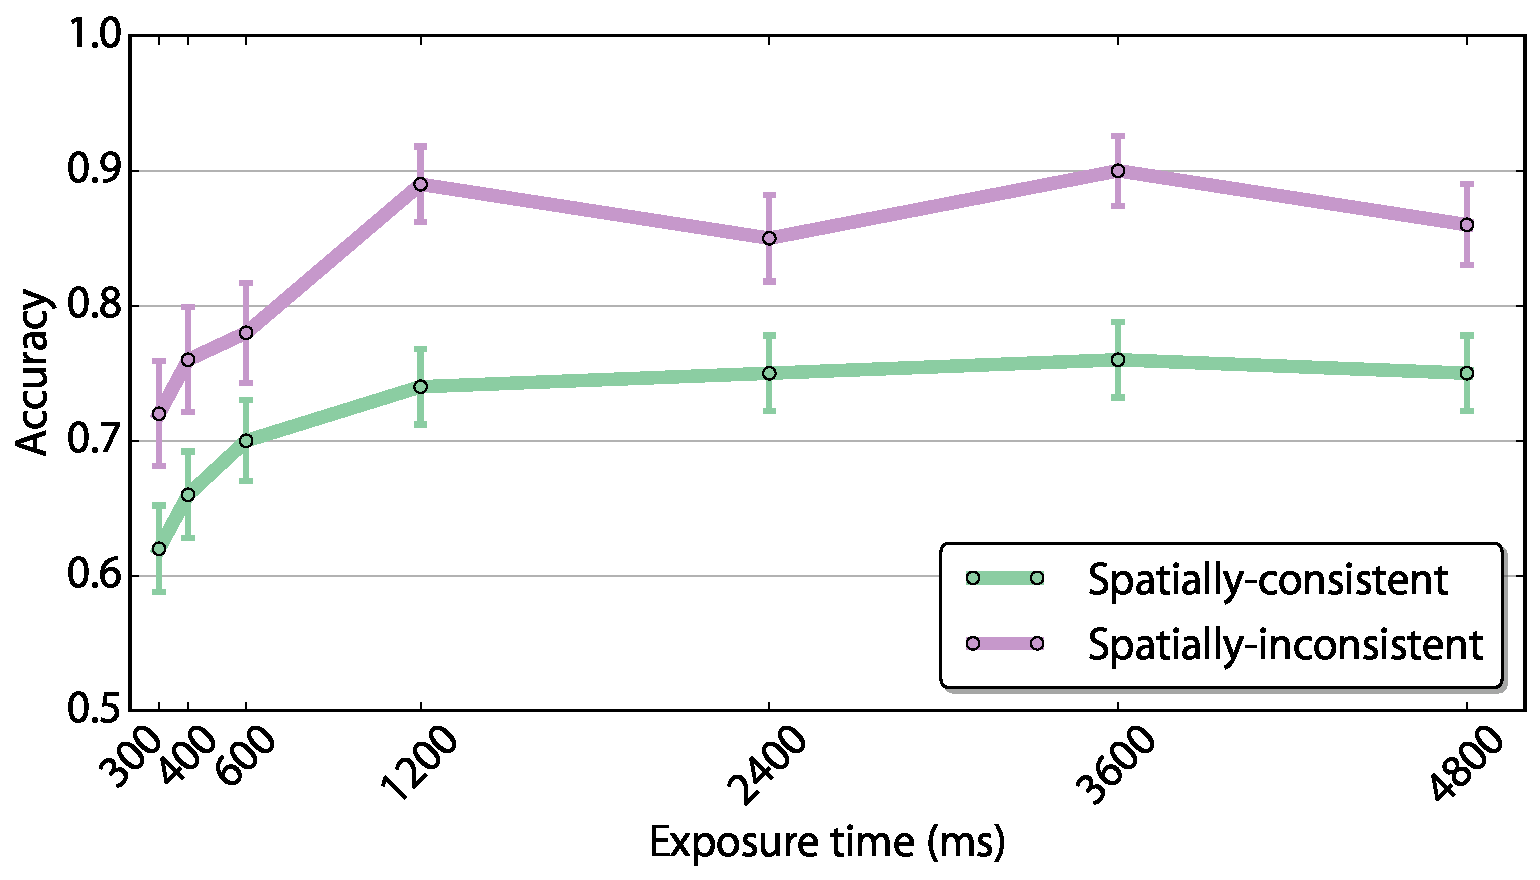
\epsfig{file=concat_dynamics.pdf, width = 0.9\textwidth}
	\caption[Time-limited pairwise comparisons across all textures, grouped by appearance and dynamics.]{Time-limited pairwise comparisons across all textures, grouped by appearance (top) and dynamics (bottom).  Shown with $95\%$ statistical confidence intervals.
	}
	\label{fig:pairwise_grouped}
	\vspace{-0.2cm}
\end{figure}

A full breakdown of the user study results by dynamic texture and 
grouping can be found in Appendix \ref{sec:full_user_study_results}.
Here some of the overall trends are discussed.

\subsubsection{Appearance-based analysis}

Based on appearance it is clear that textures with
large-scale spatial consistencies (regular, near-regular, 
and irregular textures) tend to perform poorly.
Examples being \path{flag} and \path{fountain_2} with
user accuracies of $98.9\% \pm 1.6\%$ and $90.8\% \pm 4.3\%$ 
averaged across all exposures, respectively.
This is not unexpected and is a fundamental limitation of the 
local nature of the Gram matrix representation used in the 
appearance stream which was observed in static texture synthesis 
\cite{gatys2015}.
In contrast, stochastic and near-stochastic dynamic textures 
performed significantly better as their smaller-scale local 
variations are well captured by the appearance stream, for 
instance \path{water_1} and \path{lava} which had 
average accuracies of $53.8\% \pm 7.4\%$ and
$55.6\% \pm 7.4\%$, respectively, making them both 
statistically indistinguishable from real.

\subsubsection{Dynamics-based analysis}

In terms of dynamics, the user study showed that textures with
spatially-consistent dynamics (\eg, \path{tv_static}, 
\path{water_*}, and  \path{calm_water_*}) perform 
significantly better than those with spatially-inconsistent 
dynamics (\eg, \path{candle_flame}, \path{fountain_2}, 
and \path{snake_*}), where the dynamics drastically differ 
across spatial locations.
For example, \path{tv_static} and \path{calm_water_6}
have average accuracies of $48.6\% \pm 7.4\%$ and
$63.2\% \pm 7.2\%$, respectively, while
\path{candle_flame} and \path{snake_5} have average 
accuracies of $92.4\% \pm 4\%$ and $92.1\% \pm 4\%$, 
respectively.
Overall, the two-stream model is capable of reproducing a full spectrum
of spatially-consistent dynamics.
However, as the appearance shifts from containing small-scale 
spatial consistencies to containing large-scale spatial consistencies,
performance degrades.
This was evident in the user study where the best-performing 
textures typically consisted of a stochastic or
near-stochastic appearance with spatially-consistent 
dynamics.
In contrast, the worst-performing textures consisted of
regular, near-regular, or irregular appearance with
spatially-inconsistent dynamics.

\section{Qualitative comparisons}

In this section, a qualitative comparison with the extant methods of Funke 
\etal \cite{funke2017} and Xie \etal \cite{xie2017synthesizing} is performed.
Generally, results from the proposed two-stream model are found to be qualitatively comparable or better than these methods.

To note, Funke \etal provided results on
only five textures and of those only four
are dynamic textures in the sense that their appearance
and dynamics are spatiotemporally coherent.
Their results on these sequences (\path{cranberries}, \path{flames}, 
\path{leaves}, and \path{water_5}) are included in the folder
\path{funke} under \path{dynamic_texture_synthesis/comparisons} in the supplementary material. The results from the two-stream model are included as well. An example on the \path{leaves} sequence is shown in Fig.\ \ref{fig:funke_comparison}.

\begin{figure}[t]
\begin{center}
\begin{tabular}{ >{\centering\arraybackslash} m{0.16\textwidth} || >{\centering\arraybackslash} m{0.80\textwidth} }
{target (\path{leaves})} & 
\showtexture{leaves/frame_} \\
\hline \hline
{Funke \etal \cite{funke2017}} &
\showtexture{leaves_funke/frame_} \\
\hline
{two-stream model} & 
\showtexture{leaves_output/frame_} \\
\end{tabular}
\end{center}
\vspace{-0.45cm}
\caption[Qualitative comparison with Funke \etal's \cite{funke2017} model]{Qualitative comparison with Funke \etal's \cite{funke2017} model on one of the sequences used in their work. Note that this sequence does not follow the thesis' assumption of a dynamic texture\highlight{, in the sense that the appearance and/or dynamics are not spatiotemporally homogeneous}.
(top row) Target sequence.
(middle row)
Dynamic texture synthesis when using Funke \etal's model. The model fails to capture the up-right motion of the leaves.
(bottom row)
Dynamic texture synthesis when using the proposed two-stream model. The up-right motion of the leaves is captured. Results are best viewed in video.
}
\label{fig:funke_comparison}
\end{figure}



Results are also compared on nine dynamic textures chosen to cover the full
range of the dynamics and appearance groupings introduced in the user study.
Publicly available code from Funke \etal and Xie \etal is used to produce their
results with their default parameter settings. For
Funke \etal's model, the parameters used are $\Delta{t}=4$ and
$T=12$ (recall that target dynamic textures
consist of 12 frames). For the spatiotemporal and temporal models from Xie
\etal, the parameters used are $T=1200$ and
$\tilde{M}=3$.
A comparison between the results from the proposed two-stream model, Funke
\etal's model, and Xie \etal's model
on the nine dynamic textures are included in the folder \path{xie_and_funke}
under \path{dynamic_texture_synthesis/comparisons}. An example on the \path{smoke_plume_1} dynamic texture is shown in Fig.\ \ref{fig:funke_xie_comparison}.

Note for Xie \etal, comparisons are made with their
spatiotemporal model, labelled ``Xie et al.\ (ST)'', designed for dynamic
textures with both spatial and temporal homogeneity, and their temporal model,
labelled ``Xie et al.\ (FC)'', designed for dynamic textures with only temporal
homogeneity.

\clearpage
\begin{figure}[t]
\begin{center}
\begin{tabular}{ >{\centering\arraybackslash} m{0.16\textwidth} || >{\centering\arraybackslash} m{0.80\textwidth} }
{target \break(\footnotesize\path{smoke_plume_1})} & 
\showtexture{smoke_plume_1/frame_} \\
\hline \hline
{Funke \etal \cite{funke2017}} &
\showtexture{smoke_plume_1_funke/frame_} \\
\hline
{Xie \etal \cite{xie2017synthesizing} (ST)} & 
\showtexture{smoke_plume_1_xie_st/frame_} \\
\hline
{Xie \etal \cite{xie2017synthesizing} (FC)} & 
\showtexture{smoke_plume_1_xie_fc/frame_} \\
\hline
{two-stream model} & 
\showtexture{smoke_plume_1_output/frame_} \\
\end{tabular}
\end{center}
\vspace{-0.45cm}
\caption[Qualitative comparison with Funke \etal's \cite{funke2017} and Xie \etal's \cite{xie2017synthesizing} model]{Qualitative comparison with Funke \etal's \cite{funke2017} and Xie \etal's \cite{xie2017synthesizing} models on one of the dynamic textures collected in this thesis.
(top row) Target dynamic texture.
(second row)
Dynamic texture synthesis when using Funke \etal's model.
(third row)
Dynamic texture synthesis when using Xie \etal's spatiotemporal model.
(fourth row)
Dynamic texture synthesis when using Xie \etal's temporal model.
(bottom row)
Dynamic texture synthesis when using the proposed two-stream model.
}
\label{fig:funke_xie_comparison}
\end{figure}


\clearpage

Overall, the results from the proposed two-stream model appear
qualitatively better, showing more temporal coherence and similarity
in dynamics as well as fewer spatial and temporal artifacts, such as blur and flicker, respectively.
This may be a natural consequence of the limited representation of dynamics
in both Funke \etal's and Xie \etal's models. Although the spatiotemporal model
of Xie \etal \cite{xie2017synthesizing} is able to synthesize dynamic textures
that lack spatial homogeneity (\eg, \path{bamboo} and \path{escalator}),
note that their method appears to not be able to synthesize novel dynamic textures, \ie, it
appears to faithfully reproduce the target texture, reducing the generalizability (\eg, synthesis of textures beyond the spatiotemporal extent of the input) of their approach, and thus its applicability.
 
As a consequence of jointly modelling appearance and dynamics, both methods \cite{funke2017,xie2017synthesizing} are not capable of the novel form of style
transfer that was demonstrated above. This was enabled by the factored
representation of dynamics and appearance. Furthermore, the spatiotemporal
extent of the output sequence generated by Xie \etal's
\cite{xie2017synthesizing} method is limited to being equal to the input.
The proposed approach does not share this limitation.

\section{Discussion}

This chapter provided a qualitative analysis on a variety of results obtained using the proposed two-stream model for dynamic texture synthesis, incremental texture synthesis, temporally-endless texture synthesis, and dynamics style transfer. For dynamic texture synthesis, it was shown that both the appearance and dynamics streams were required to synthesize dynamic textures that matched both the framewise appearance of the target and its dynamics. For incremental texture synthesis, it was shown that incrementally synthesized dynamic textures exhibited no divergence or degradation when compared to those synthesized using the typical batch process. For temporally-endless texture synthesis, it was shown that the synthesized dynamic textures exhibited no apparent temporal discontinuity between the last and first frames. For dynamics style transfer, it was shown that the dynamics of one dynamic texture can be successfully combined with the appearance of another, under the stipulation that the appearance and dynamics targets came from textures similar in scale and semantics.

Additionally, a large-scale user study was performed to quantitatively evaluate the realism of dynamic textures synthesized by the proposed model by comparing synthesized results with their respective targets. An evaluation on a baseline version of the model was performed as well. Overall, dynamic textures synthesized by the two-stream model were able to fool users $33.9\% \pm 2.5\%$ of the time for brief exposures. In contrast, dynamic textures synthesized by the baseline model were able to fool users $10.2\% \pm 1.8\%$ of the time.

Finally, a qualitative comparison with two extant methods for dynamic texture synthesis was performed. Overall, the results from the proposed two-stream model were shown to be qualitatively better than the compared methods, showing more temporal coherence and similarity in dynamics as well as fewer spatial and temporal artifacts. Furthermore, the other methods were shown to lack the capability of the novel dynamics style transfer shown by the proposed two-stream model.

% qualitative results
  % dynamic texture synthesis
  % incremental texture synthesis
  % temporally-endless texture synthesis
  % dynamics style transfer
% user study
% qualitative comparisons